\subsubsection{animation}
    Benötigte Klassen sowie ihre Schnittstellen zu dem Interface, dass bereits von der 
    JMonkeyEngine vorgegeben wird um (eine/mehrere) Animationen zu realisieren. \par
    \begin{figure}[htbp]
        \centering
        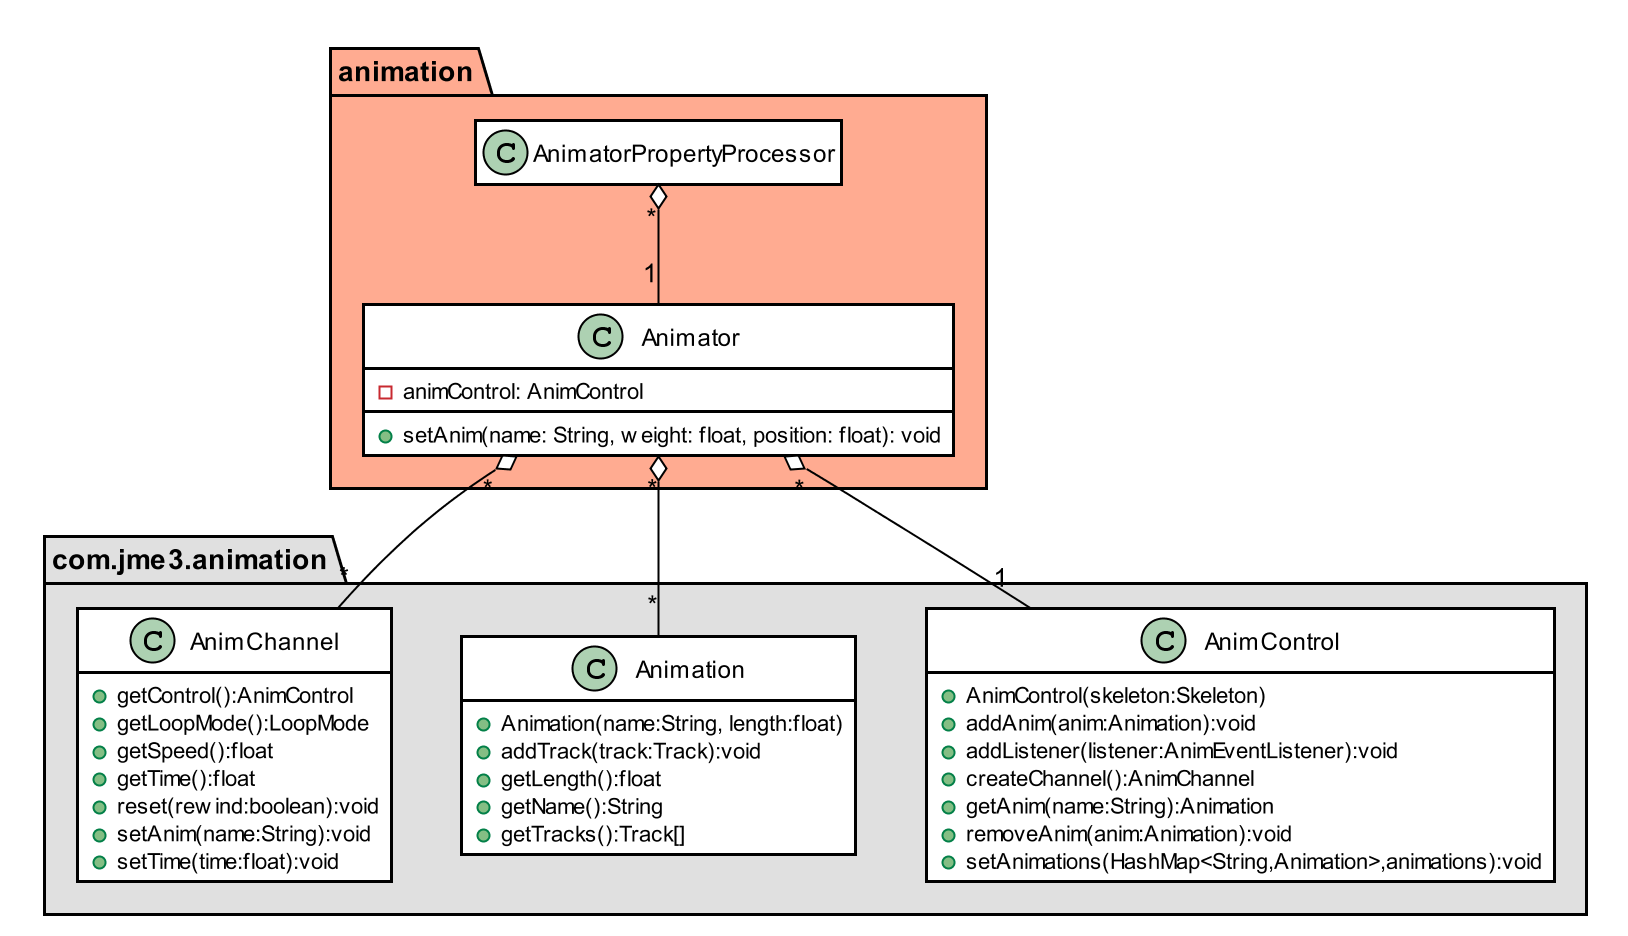
\includegraphics[width=1\linewidth]{InGameGrafik/Bilder/animation.png}
        \caption{Klassendiagramm animation}
    \end{figure}
    \paragraph{\underline{Animator}} \mbox{}\par
                Klasse zur Steuerung einer Animation.\par
                
                \textbf{Attribute}
                \begin{itemize}
                    \item  \textit{animControl} 
                        \begin{leftbar}[0.9\linewidth]
                        Kontroller zur Steuerung der Animation.  
                        \end{leftbar}
                \end{itemize}

                \textbf{Methoden}					
                \begin{itemize}
                    \item  \textit{setAnim(String name, float weight, float position): void}
                        \begin{leftbar}[0.9\linewidth]
                            Setzt eine Animation auf der Scene.\\
                            \textbf{@param name} Name der Animation.\\
                            \textbf{@param weight} "Gewicht der Animation".\\
                            \textbf{@param position} Position der Animation innerhalb der Scene.
                        \end{leftbar}   
                \end{itemize}
\pagebreak